\documentclass[]{scrartcl}
\usepackage{graphicx}
\usepackage{color}
\usepackage{german}
\usepackage{hyperref}
\usepackage{calc} 
\usepackage{enumitem}
%\pagestyle{headings}

% customize dictum format:
\usepackage[T1]{fontenc}
\setkomafont{dictumtext}{\itshape\small}
\setkomafont{dictumauthor}{\normalfont}
\renewcommand*\dictumwidth{\linewidth}
\renewcommand*\dictumauthorformat[1]{--- #1}
\renewcommand*\dictumrule{}
\newcommand{\todo}[1]{\textcolor{red}{TODO: #1}\PackageWarning{TODO:}{#1!}}

\begin{document}

\title{
	\includegraphics*[width=0.75\textwidth]{images/hu_logo.png}\\
	\vspace{24pt}
	Studienbeginn und Orientierung}
\subtitle{Block WS 16/17\\
          Humboldt Universit"at zu Berlin}
\author{Lennard Wolf\\
        \href{mailto:lennard.wolf@student.hu-berlin.de}{lennard.wolf@student.hu-berlin.de}}
\maketitle
\begin{abstract}

Studienprobleme? Ich habe doch gerade erst mit dem Studium angefangen. Aber nachdem die erste Euphorie verflogen ist, kann es wichtig sein zu wissen, welche L"osungen es gibt, wenn es doch mal nicht so l"auft, wie man will. Was mache ich, wenn ich durch den dritten Pr"ufungsversuch falle oder mein Studienfach nicht meinen Erwartungen entspricht? An diesem Tag laden wir Sie zu folgenden Veranstaltungen ein, die Sie auf ein erfolgreiches Studium vorbereiten:

Informationen zum Studium, Studienaufbau von Compass-Tutor -- Erfolgreich studieren - aber wie? -- F"uhrung Campus Mitte -- Vortrag \emph{Stressbew"altigung - Stress erkennen, vermeiden, bew"altigen}

\end{abstract}
\newpage

\tableofcontents
\newpage

\section{Studienorganisation \& CMS}

\subsection{Agnes}
\url{hu.berlin/agnes}
\newline

Vor Semesterbeginn sollte in dem Vorlesungsverzeichnis Agnes eine Belegung ausgetestet werden indem die Kurse \emph{vorgemerkt} werden, dann der Stundenplan angeschaut wird und dann auf \emph{belegen} und dann auf \emph{speichern} geklickt wird.

Leistungsnachweise sind hier einzusehen sowie der resultierende Notenspiegel. Adresse kann hier ge"a"andert werden.

\subsection{Moodle}
\url{hu.berlin/moodle}
\newline

Das Moodle ist f"ur Kursmaterialen und -dateien da, d.h. f"ur das Austeilen von Aufgaben. Zudem gibt es kursspezifische Foren. Da "uber das Moodle Mails verschickt werden, sollte die e-mail Adresse hier spezifiziert sein! Kurse werden im Moodle am besten "uber die Kursnummern gefunden.

Anmelden geht mit dem allgemeinen HU-Account. 

\subsection{Amor}
\url{hu.berlin/amor}
\newline

Oder auch: die allgemeinen Internetdienste (eduroam, VPN etc.).
Mit dem VPN lassen sich jstor, wiley, springerlink etc. erreichen.

\subsection{Unibibliotheken}

Der Studierendenausweis ist gleichzeitig aus der Benutzerausweis f"ur die Bibliotheken. Die Benutzernummer steht entsprechend auf dem Studierendenausweis (HUHS...). Das vorl"aufige Passwort ist die PLZ mit dem ersten Buchstaben des Strassennamens. Lizenzen f"ur die Suche in professionellen DBs nur "uber eduroam oder VPN.

Man sollte sich wenn man online einen Text gefunden hat den man sich ausleihen will, die Signatur aufschreiben bevor man an den Ausleihautomaten in der Bib geht. Deutschlandweite Fernleihe ist m"oglich, mit KOBV berlinweit. Schließf"acher mit Mensacard. Gruppenarbeitsr"aume sind kostenlos reservierbar.

"Offnungszeiten Grimm-Zentrum:

\begin{description}[leftmargin=!,labelwidth=\widthof{\bfseries Mo - Fr}]
  \item[Mo - Fr]  8h -- 24h
  \item[Sa - So] 10h -- 22h
\end{description}

\newpage


\section{Erfolgreich im Studium}

33\% der Studierenden brechen ihr Studium ab. Um das f"ur sich zu umgehen ist es wichtig, sich von Anfang an mit dem neuen Umfeld vertraut zu machen, sich zu organisieren, Pr"ufungszeitr"aume immer gut abzusch"atzen, lange im vorraus planen und sich konkrete Ziele zu stecken. HiWi Jobs sind sinnvoll um tiefere Einblicke zu bekommen. Es gibt Studienfinanzierungsberatungsstellen. Gibt es also Stipendien f"ur Philosophen?

Bei sehr starken Zweifeln empfiehlt es sich den \emph{prevdrop} Test der HU zu machen.

\begin{figure}[h]
	\centering
	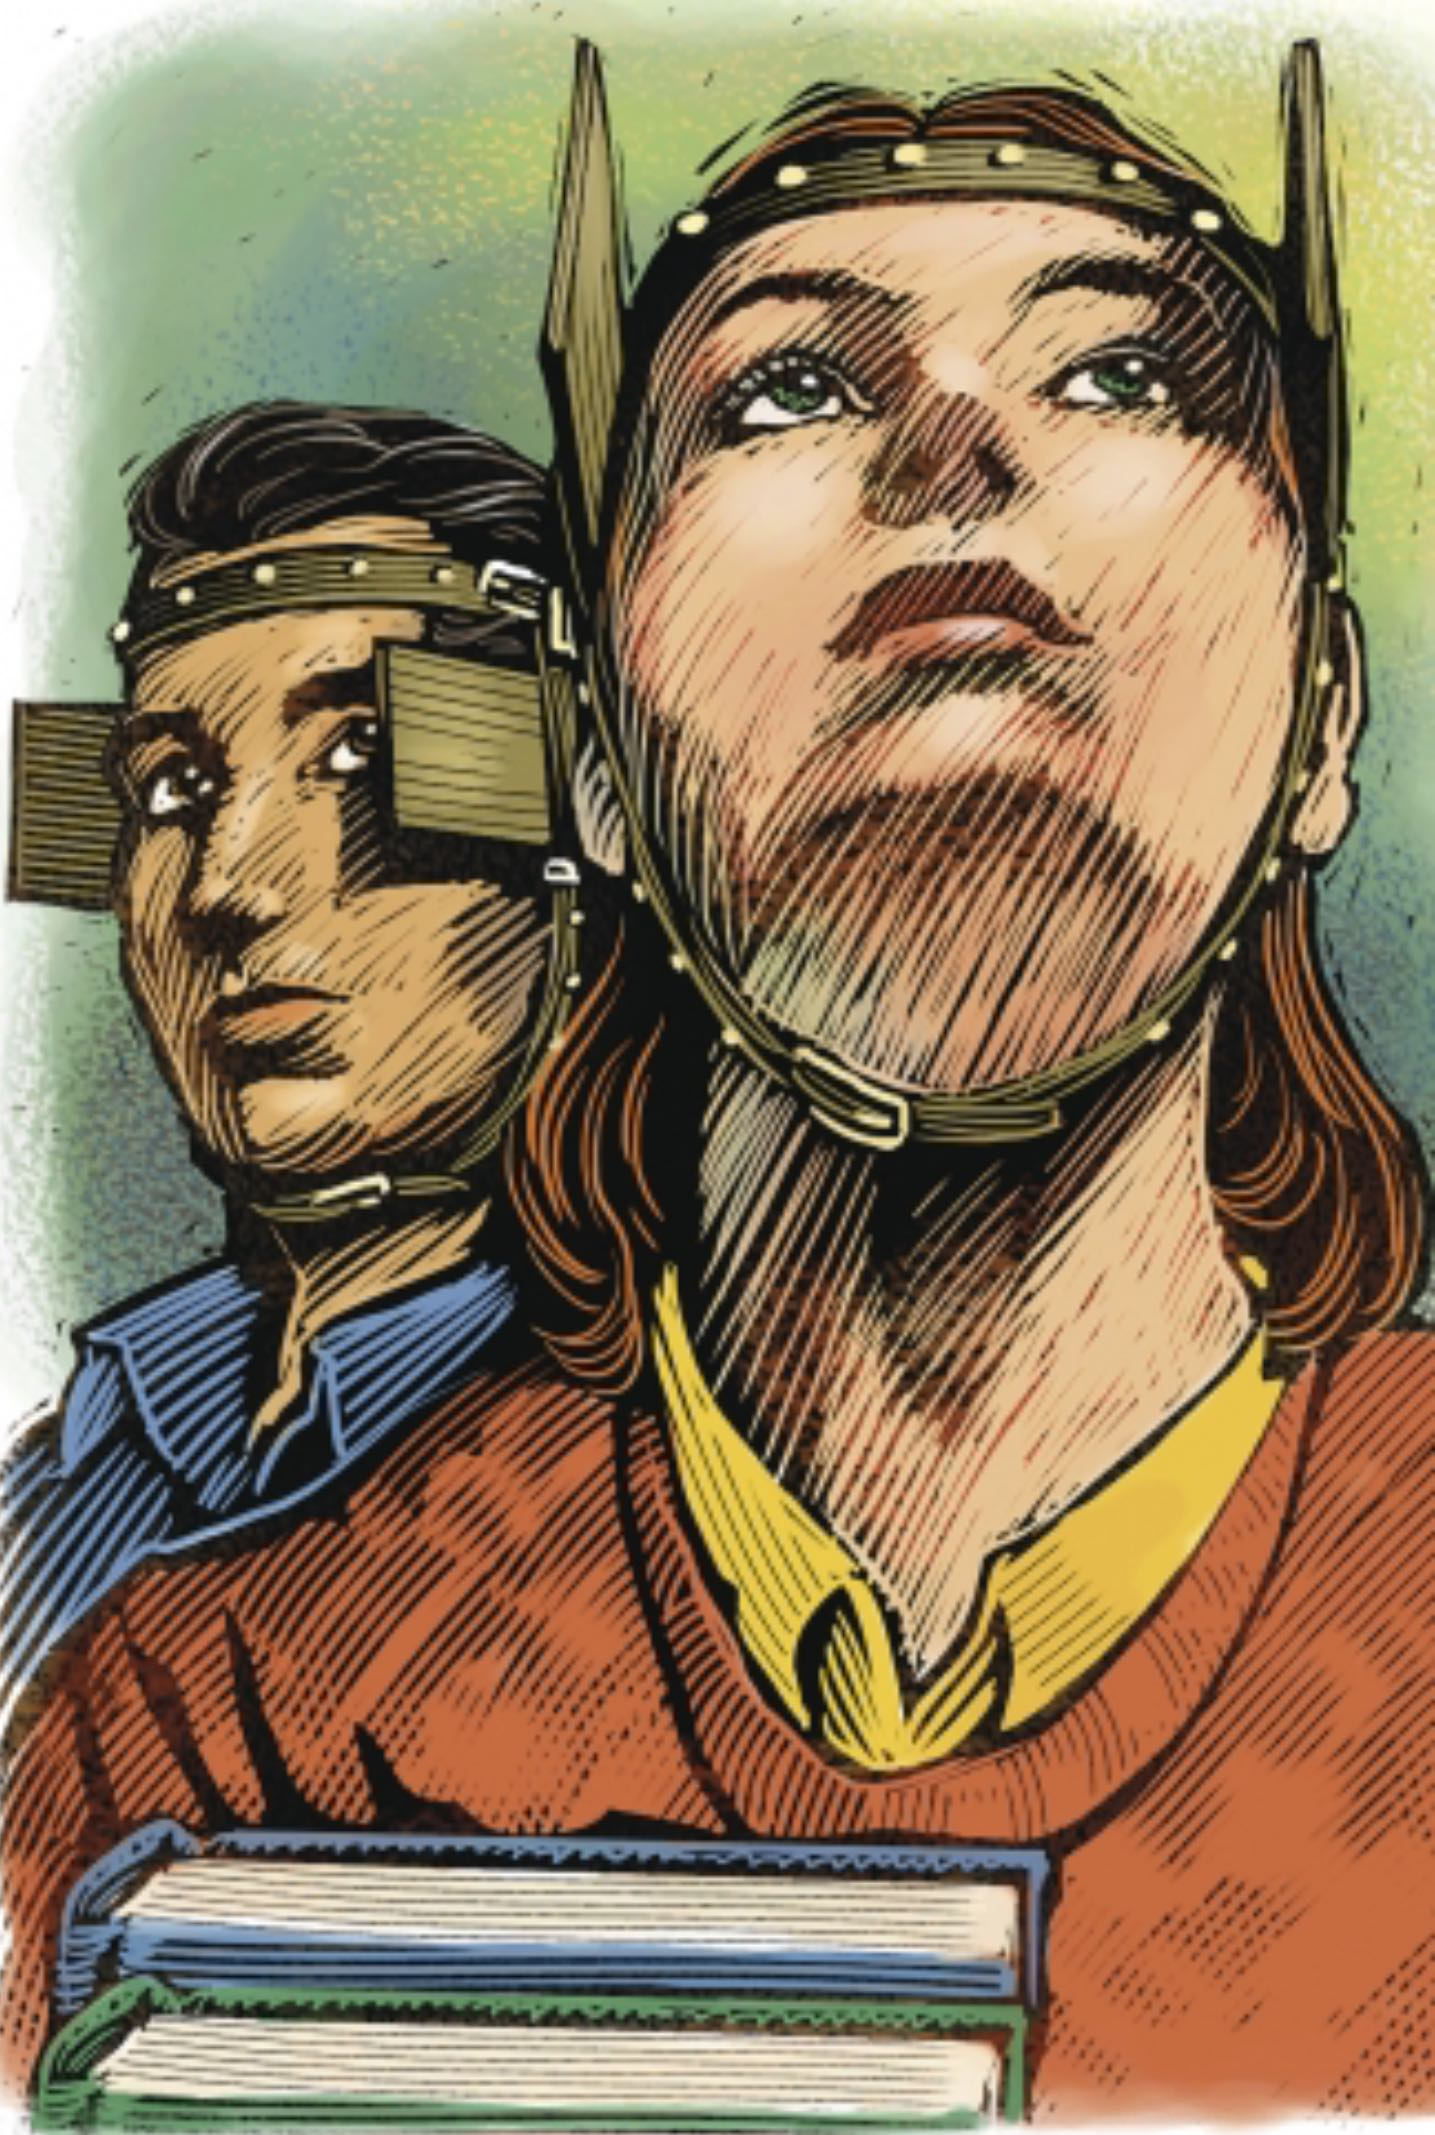
\includegraphics[width=0.3\textwidth]{images/studienorga/scheu.jpg}
	\caption{Scheuklappenstudierende}
	\label{fig:sess}
\end{figure}

\subsection{10 Tipps}

\begin{enumerate}
  \item Pr"ufungsordnung lesen!
  \item Agnes und Moodle fr"uh einrichten
  \item Einf"uhrungsveranstaltungen besuchen
  \item Ansprechpartner identifizieren und treffen
  \item Termine im "Uberblick haben
  \item Studium -- Freit in Balance haben
  \item Lernmethoden herausfinden und testen
  \item Campusangebote nutzen
  \item Pr"ufungsordnung lesen!
\end{enumerate}

\section{Stressbew"altigung}

\subsection{Was ist Stress?}

Der Stressbegriff stammt aus der Materiallehre und wurde erst in den 50ern in Verbindung zu Mensch und Tier gebracht. Stress wird durch so genannte \emph{Stressoren} ausgel"ost.

80\% der Deutschen finden ihr Leben stressig. Aber Stress muss nicht nur negativ sein, denn er ist dazu da, uns schnell auf einen Wechsel der Umgebung einzustellen. Stress kann als \emph{Aktivierungsreaktion} verstanden werden, er ist eine Antwort auf Belastung und erh"oht entsprechend die Leistung. Es gibt \emph{Eu-Stress} und \emph{Dis-Stress}, wobei der erste positiv, also motivierend und fordernd ist, w"ahrend der letztere negativ ist, da die Bew"altigungsm"oglichkeit "ubersteigt wird und der Organismus nicht mehr voll funktionsf"ahig ist.

Der Verlauf einer Stressreaktion verl"auft wie folgt: $Alarm \rightarrow Orientierung \rightarrow Aktivierung \rightarrow Anpassung \rightarrow Erholung \rightarrow "Uberforderung \rightarrow Ersch"opfung $


\textbf{Warnzeichen: } Reizbarkeit, Aggression, weinerlich, keine Konzentration, unn"otige Fehler, Schlafst"orungen, Kopfschmerzen, Herz-Kreislauf-Probleme 

\textbf{Ebenen:      } kognitive, emotionale, vegetativ hormonische, muskul"are

Auf jede Anspannung muss Entspannung folgen!


\subsection{Stressoren}

Stressoren sind Anforderungen die von innen (\emph{Ich muss das perfekt machen!}) wie von au\ss en (Krankheit, L"arm) kommen k"onnen. 

Der K"orper reagiert auf diese durch \emph{Mobilmachung}, indem die Hormone Adrenalin (\emph{Fight or Flight}) und Kortisol (Sauerstoff im K"orperverteilen f"ur h"oheres Energiepotenzial) freigesetzt werden. Da der K"orper nun erwartet aktiviert zu werden (und nicht nur in der Bibliothek zu sitzen) muss zum Ausgleich Sport getrieben werden! Zudem sollte erw"ahnt werden, dass Menschen die unter Stress stehen schlechtere Entscheidungen f"ur sich treffen und sich entsprechend tendenziell zu wenig bewegen, ausgleichen und schlecht ern"ahren. 

Abbildungen \ref{fig:stressdosis} und \ref{fig:stress} zeigen die sinnvolle, sogenannte \emph{mittlere Stressdosis}.

\begin{figure}[h]
	\centering
	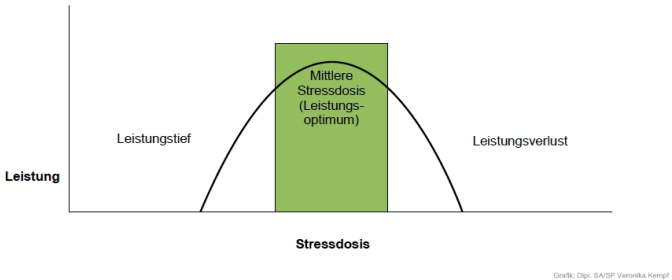
\includegraphics[width=0.68\textwidth]{images/studienorga/stressdosis.jpg}
	\caption{Mittlere Stressdosis}
	\label{fig:stressdosis}
\end{figure}


\begin{figure}[h]
	\centering
	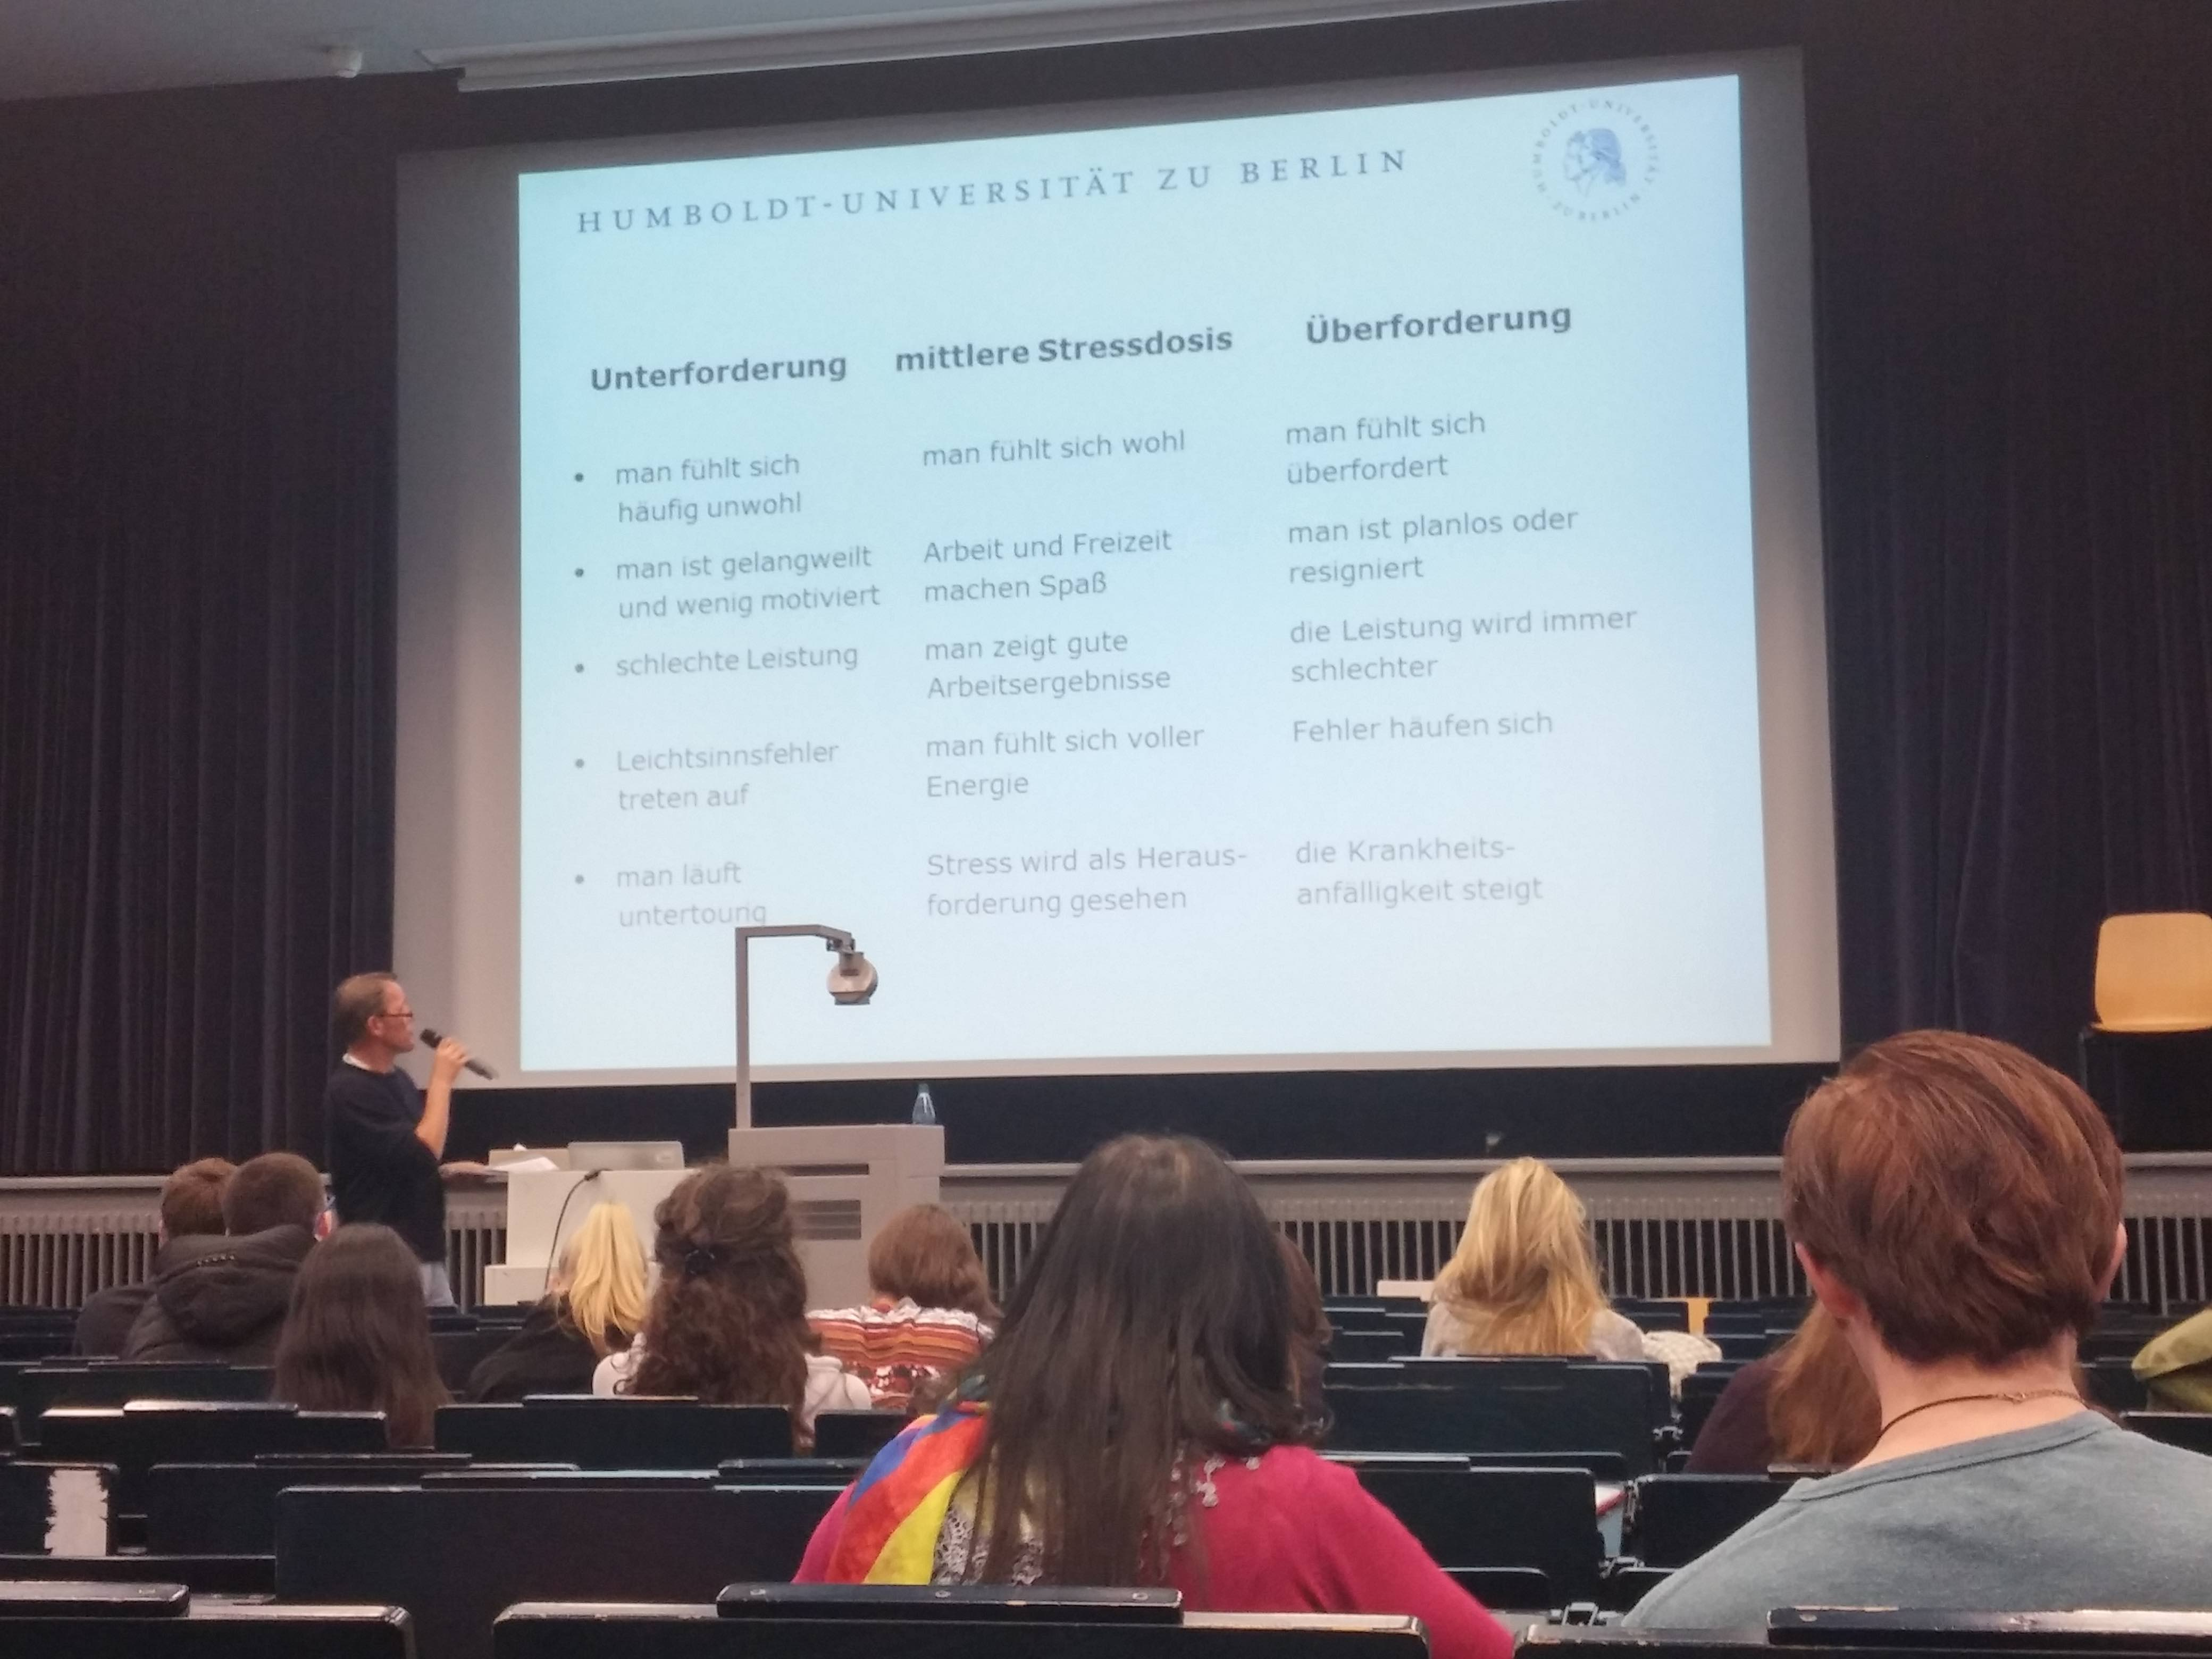
\includegraphics[width=0.82\textwidth]{images/studienorga/stress.jpg}
	\caption{Kurs Stressbew"altigung}
	\label{fig:stress}
\end{figure}

Stressoren k"onnen \emph{objektiv} und \emph{subjektiv}. Erstere sind also f"or alle "uhnlich stressend, zB eine große Menge von Arbeit oder eine unruhige Umgebung. Jedoch kann eine pers"onliche Haltung einen Umstand zu einem Stressoren machen, indem eine unangemessene Bewertung der Lage wegen pers"onlicher Haltungen vorgenommen wird (\emph{Ich muss es allen recht machen!}). Es kann auf beide Formen entweder \emph{reaktiv} oder \emph{proaktiv} reagiert werden: Im ersten Fall nimmt die betroffene Person eine unterw"urfige Stellung ein und gibt auf oder l"asst sich unterkriegen. Eine proaktiv handelnde Person wiederum w"urde versuchen die Stressoren zu identifizieren, und daraufhin zu reduzieren oder ganz zu eliminieren. Sprache spielt zudem auch eine tragende Rolle: Sich zu sagen \emph{Ich nehme mir dir Zeit!} anstatt \emph{Ich muss mir die Zeit nehmen...} kann einen gro\ss en Einflu\ss auf unser Bild unseres Lebens haben. 

\subsection{Bew"altigung}

Es empfiehlt sich, sich eine \emph{regenerative Stresskompetenz} anzueignen. Folgende M"oglichkeiten treiben die Erholung voran: 

\begin{itemize}
    \item Erholungsaktivit"aten aus stressfreien Zeiten beibehalten
    \item Sich sagen \emph{Schlu\ss~ f"ur heute!}
    \item K"orperliche Entspannung durch Meditation und Yoga
    \item Soziale Kontakte pflegen
    \item Nicht w"ahrend des Essens arbeiten
  \end{itemize}

Nat"urlich darf nicht vergessen werden, dass sich pr"aventives Verhalten auch auszahlt:

\begin{itemize}
    \item Tagespl"ane erstellen (basierend auf Wochenpl"anen)
    \item Wichtige und anstrengende Dinge zuerst abhaken
    \item Checklisten pflegen und Erledigtes anerkennen
  \end{itemize}


\section{Neue Begriffe}

\begin{description}[leftmargin=!,labelwidth=\widthof{\bfseries Blockveranstaltung}]
  \item[Blockveranstaltung] Veranstaltung die nur ein bis wenige Male stattfindet und dann in einem Block, zB Samstag von 8 bis 19 Uhr
  \item[ct] \emph{con temporare} -- akademisches Viertel
  \item[CMS] Computer- und Medienservice
  \item[MAP] \textbf{M}odul \textbf{A}bschluss \textbf{P}r"ufung
  \item[jstor] Digitale Bibliothek f"ur Akademische Journale und B"ucher
  \item[Wiley] Digitale Bibliothek f"ur Akademische Journale im naturwissenschaftlicehn Bereich
  \item[Springerlink] Online-Informationsdienste f"ur naturwissenschaftliche, technische und medizinische B"ucher und Zeitschriften
  \item[KOBV] (Kooperativer Bibliotheksverbund Berlin-Brandenburg) Katalog der Berliner und Brandenburger Bibliotheken
\end{description}



\section{Notes to Self}

\begin{itemize}
    \item Mehr als 30 Punkte pro Semester planen
    \item Matrikelnummer lernen
    \item Erstitage: Fragen wann/wie Pr"ufungsanmeldung zu passieren hat
    \item Hauptfach geht immer vor
    \item TANs sind f"ur Pr"ufungsanmeldungen (1 pro 1)
    \item vllt mit Endnote etc. vertraut machen
    \item Erasmusb"uro?
    \item Samstags immer nachbereiten, lesen und hinterfragen

  \end{itemize}
\newpage
\section{Anhang}

\begin{figure}[h]
	\centering
	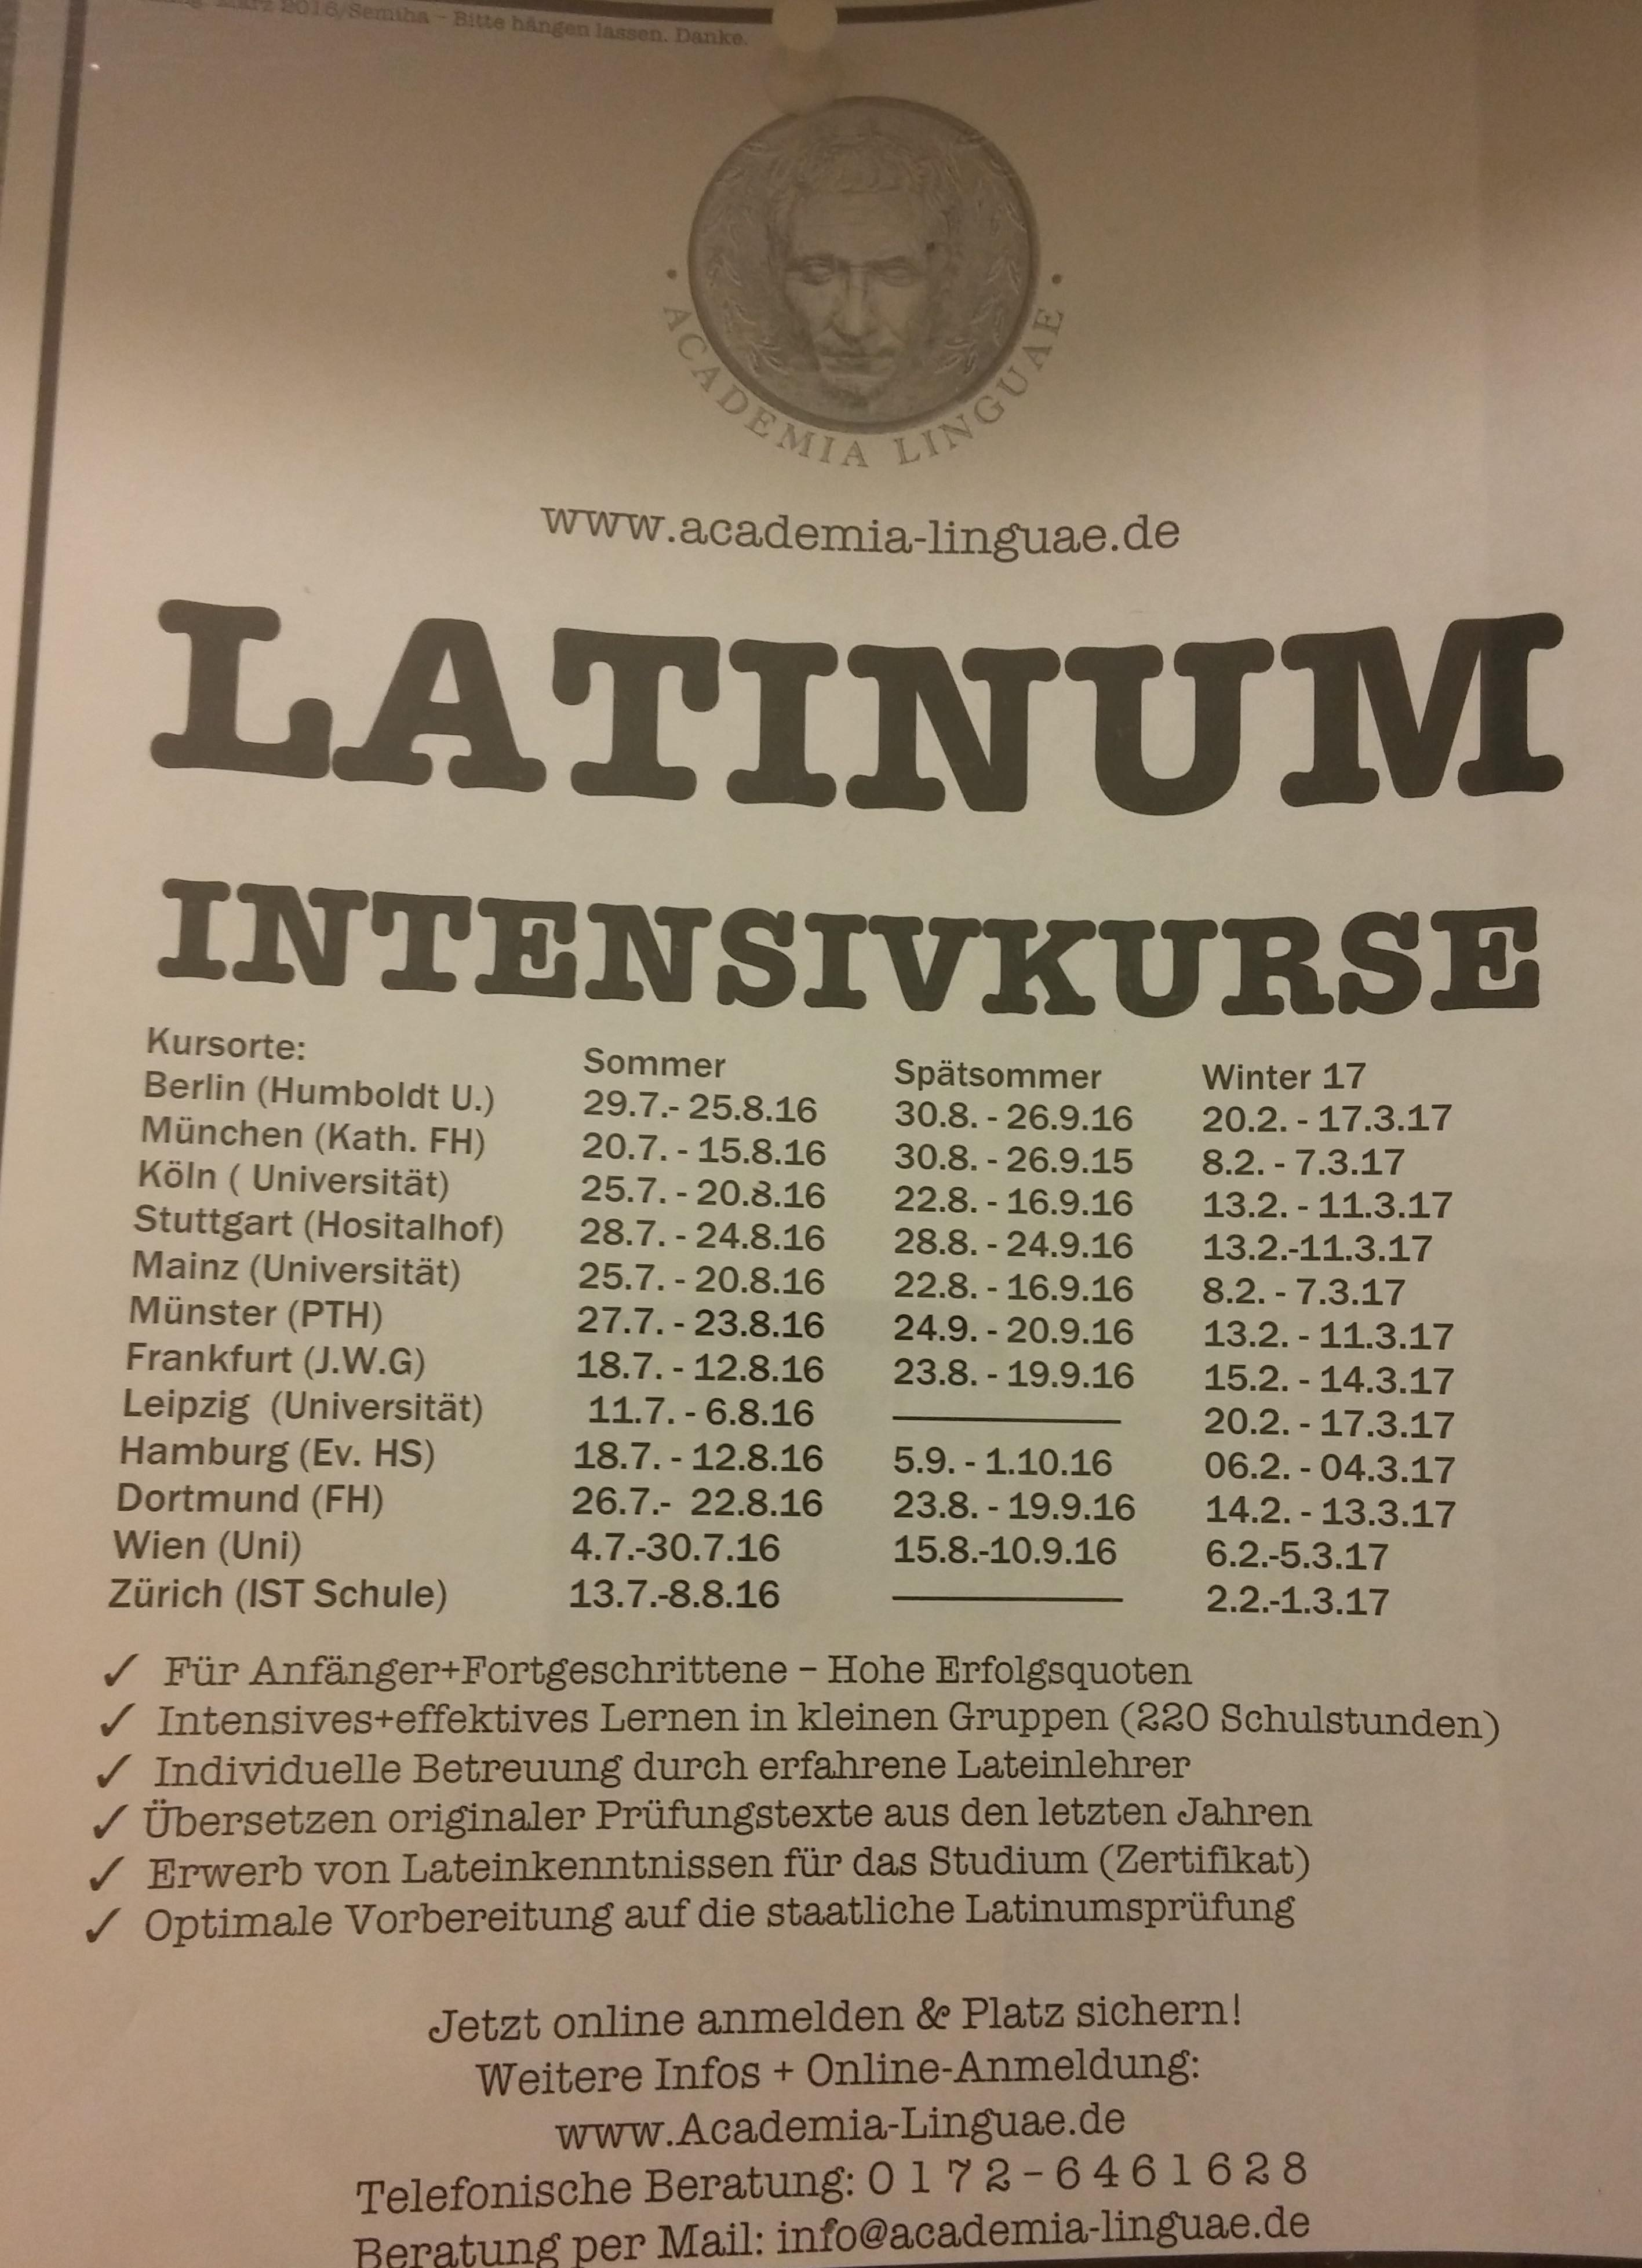
\includegraphics[width=0.7\textwidth]{images/studienorga/latin.jpg}
	\caption{Latinum}
	\label{fig:sts}
\end{figure}


\begin{figure}[h]
	\centering
	
\includegraphics[width=0.7\textwidth]{images/studienorga/stip.jpg}
	\caption{DeutschlandStipendium}
	\label{fig:strss}
\end{figure}

\end{document}
